\chapter{\textit{Master-Slave}}\label{sec:master_slave}

Este padrão apresenta um sistema regido por um mestre capaz de obter informações de agentes do grupo, criar planos e atribuir tarefas a agentes individuais, a fim de assegurar a coerência global.


\begin{description}
  \item[Nome do padrão:] \textit{Master-Slave}.
    \item[Referências:]    \citeonline{aridor1998agent}.
    \item[Categoria:] \textit{Simple structure}.
    \item[Problema:] ocorre quando um agente mestre, (ou \textit{Master}), precisa executar uma tarefa em paralelo com outras tarefas para as quais é responsável. Ocorre também quando este agente deseja executar uma tarefa em um destino remoto.
    \item[Solução:] Quatro classes participam deste padrão. A Figura \ref{fig:master_sl_diagrama} ilustra suas relações estruturais.
    \begin{itemize} 
    \item \textbf{\textit{Master}:} define um esqueleto de um agente mestre, usando métodos abstratos para serem substituídos na classe \textit{Concrete-Master}.
    \item \textbf{\textit{Slave}:} define um esqueleto de um agente escravo, usando métodos abstratos para serem sobrescritos pela classe \textit{ConcreteSlave}.
    \item \textbf{\textit{ConcreteMaster}: }implementa métodos abstratos da classe \textit{Master}.
    \item \textbf{ConcreteSlave}: implementa métodos abstratos da classe \textit{Slave}.
    \end{itemize}


\begin{figure}[h!]
    \centering
    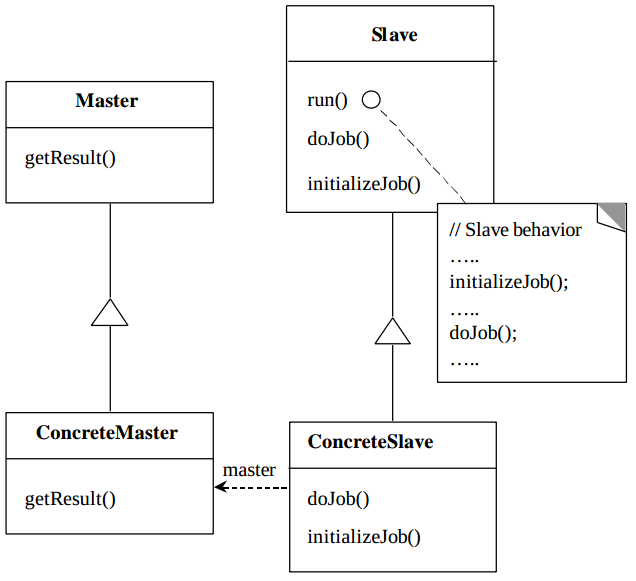
\includegraphics[scale=0.35]{figuras/master_slave/master_sl_diagrama.png}
    \caption{Participantes do padrão \textit{Master-Slave}. Fonte: \citeonline{aridor1998agent}}
    \label{fig:master_sl_diagrama}
\end{figure}

Primeiramente, o agente \textit{Master} cria um agente \textit{Slave}. Este, move-se para um \textit{host} remoto e executa a tarefa para o qual foi designado. Em seguida, retorna com o resultado da tarefa para o agente \textit{Master}.


\item[Modelagem:] este padrão pode ser representado pela Figura \ref{fig:master_sl_diagrama_sequencia}.

\begin{figure}[h!]
    \centering
    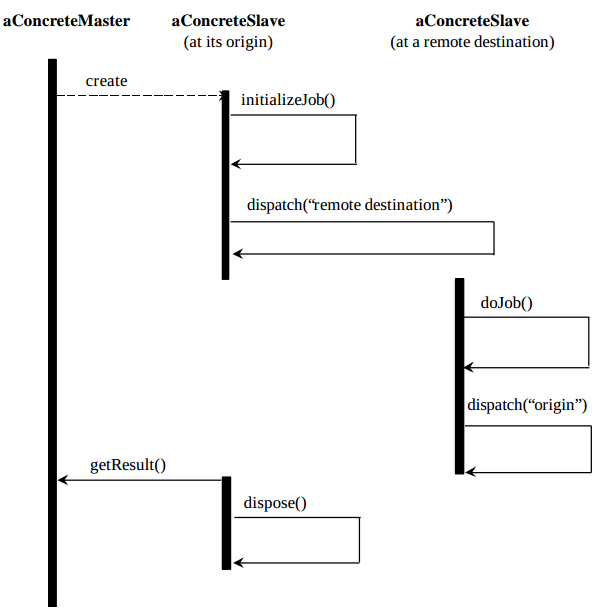
\includegraphics[scale=0.4]{figuras/master_slave/diagrama_sequencia.png}
    \caption{Diagrama de sequência do padrão \textit{Master-Slave}. Fonte: \citeonline{aridor1998agent}.}
    \label{fig:master_sl_diagrama_sequencia}
\end{figure}



    \item[Exemplo:] O exemplo a seguir baseia-se em um aplicativo que fornece uma GUI para inserir dados e exibir os resultados intermediários de uma tarefa específica a ser realizada remotamente.

Com um único agente para fornecer a GUI e executar essa tarefa, não será possível manter a GUI depois que o agente viajou de sua origem para um destino remoto. A alternativa é adotar um agente escravo para que se mova para outro destino, execute a tarefa atribuída, envie os resultados intermediários e, finalmente, retorne com o resultado da tarefa ao agente mestre. Este, por sua vez, exibe o resultado para seu cliente.

A ideia chave do padrão é usar classes abstratas, mestre e escravo, para localizar as partes invariantes de delegar uma tarefa entre agentes mestres e escravos, consistindo em três principais comportamentos: (i) despachar um escravo de um lado para outro para outros destinos; (ii) iniciar a execução da tarefa, e (iii) lidar com exceções ao executar a tarefa.

Os agentes mestres e escravos são definidos como subclasses de mestre e escravo. Apenas partes variáveis, como a descrição de como a tarefa deve ser executada e como o agente mestre deve lidar com o resultado da tarefa, são implementadas. Na prática, a classe \textit{Master} possui um método abstrato \textit{getResult()} para definir como lidar com o resultado da tarefa.

A classe \textit{Slave} tem dois métodos abstratos, \textit{initializeJob()} e \textit{doJob()}, que definem as etapas de inicialização a serem executadas antes que o agente viaje para um novo destino e a tarefa a ser executada, respectivamente. Ambas as classes são definidas em termos desses métodos. O código a seguir mostra a classe \textit{Slave} implementada como um \textit{Aglet}.

\begin{lstlisting}[firstnumber=1]
public abstract class Slave extends Aglet {
    Object result = null
 
    public void onCreation(Object obj) {
        // Called when the slave is created.Gets the
        // remote destination, a reference to the master
        // agent, and other specific parameters.
    }
 
    public void run () {
        // At the origin:
        initializeJob();
        dispatch(destination); // Goes to destination
        // At the remote destination:
        doJob(); // Starts on the task.
        result=...;
        // Returns to the origin.
        // Back at the origin.
        // Delivers the result to the master and dies.
        dispose();
}
\end{lstlisting}

\item[Implementação:] a fim de demonstrar este padrão, é utilizado um contexto de fechamento de caixa de uma loja. Todos os detalhes da implementação, configuração de ambiente e passos para execução são descritos no Apêndice \ref{appendix:master_slave}.

\end{description}



